\graphicspath{{./figures}}

\section{PocketQube Unit Antenna}
\subsection{Mechanical Considerations}
Since the system is constrained close to the 433 MHz band (due to the radiosonde link), the wavelength of interest is relatively large (693 mm), and one half of a half-wavelength dipole is around 173 mm. Special consideration would be needed to fit this onto the planned PocketQube length of 150 mm. For the planned prototype balloon satellite launch, it is therefore decided to design a half-wavelength dipole, and allow it to simply protrude out the ends of the PocketQube housing from launch. Recommendations for future projects are given in Section \ref{sec:future_work} (such as designing a deployable antenna).

\subsection{Simulation Design and Matching}
A simple 1.5 mm metal wire will be used for the dipole due to its availability, which will be fed by a coaxial cable. The design parameters for the dipole are $L_\lambda$ (the total dipole length relative to lambda), $F_{\textnormal{gap}}$ (the gap distance of the feed), and $F_{length}$ (the length of the feed). A fixed gap distance of $F_{\textnormal{gap}} = \SI{5}{mm}$ was decided on, as it was assumed to not have a large impact on the results if it kept sufficiently small.

\begin{figure}[!htb]
  \begin{minipage}{.38\textwidth}
    \centering
    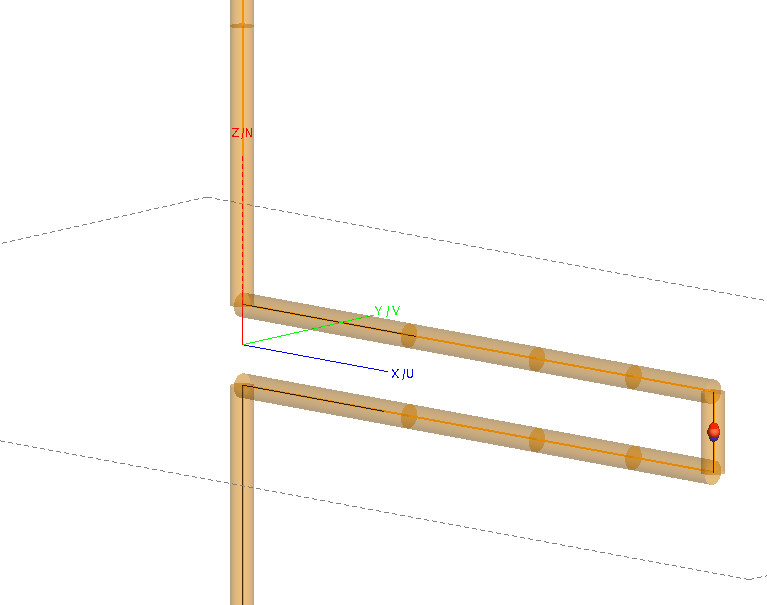
\includegraphics[width=0.95\linewidth]{dipole1_modelMesh}
    \caption{Dipole Model}
    \label{fig:dipole1_modelMesh}
  \end{minipage}
  \begin{minipage}{.6\textwidth}
    \centering
    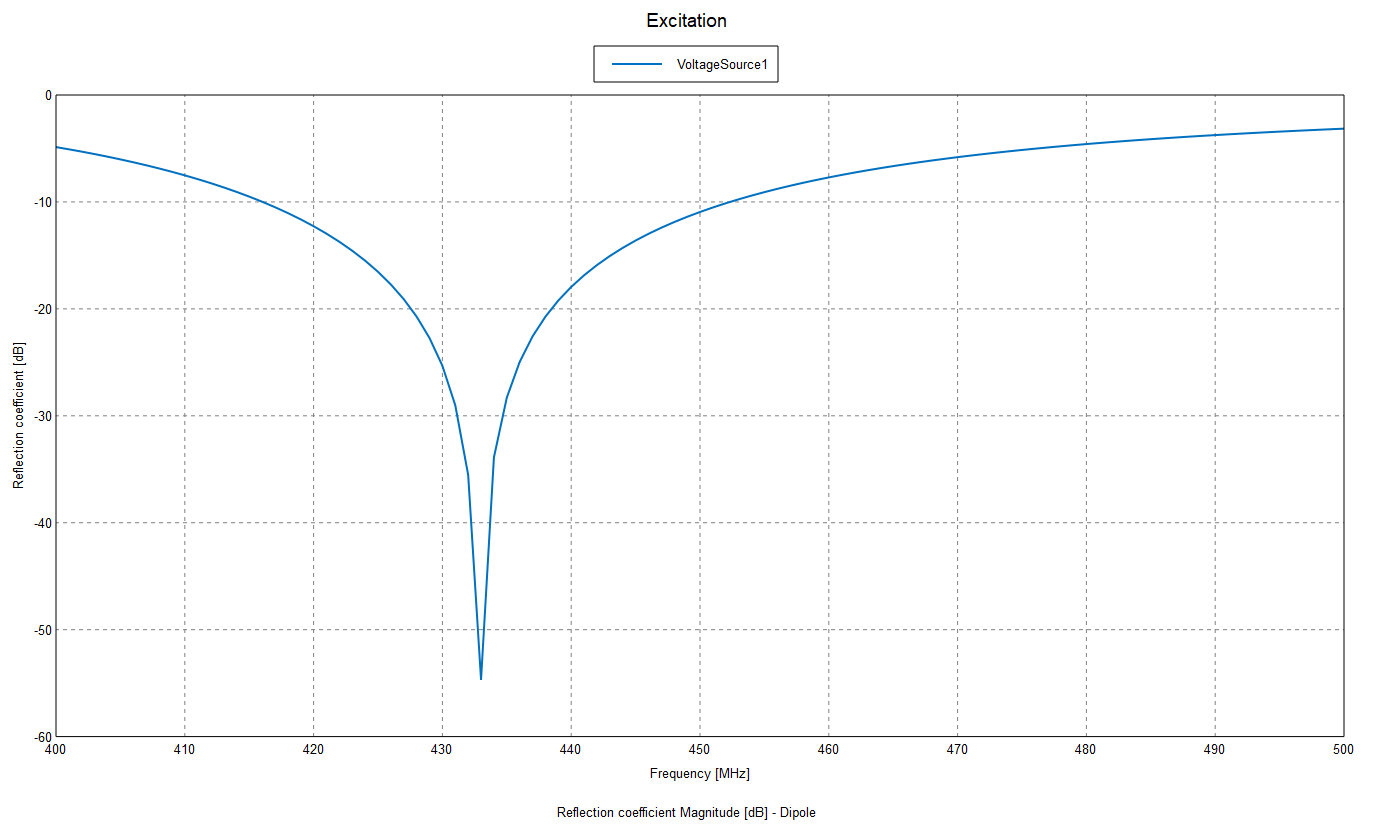
\includegraphics[width=0.9\linewidth]{dipole1_returnLoss}
    \caption{Simulated $0.45 \lambda$ Dipole Return Loss vs Frequency}
    \label{fig:dipole1_returnLoss}
  \end{minipage}
\end{figure}

The FEKO model in Figure \ref{fig:dipole1_modelMesh} was used. The optimiser was used to calculate the optimal dipole length and feed length that would minimize the return loss for $f = \SI{433}{MHz}$ at a feed impedance of $\SI{50}{\ohm}$. The resultant parameters are found to be $L_\lambda = 0.45$ ($L = \SI{312}{mm}$) and $F_{\textnormal{length}} = \SI{39.0}{mm}$. The optimised return loss as a function of frequency is shown in Figure \ref{fig:dipole1_returnLoss}. The radiation pattern was found to be the classic ``donut" shape, with a maximum directivity of 2.1 dBi.